\begin{frame}{Nextcloud}
	\begin{center}
		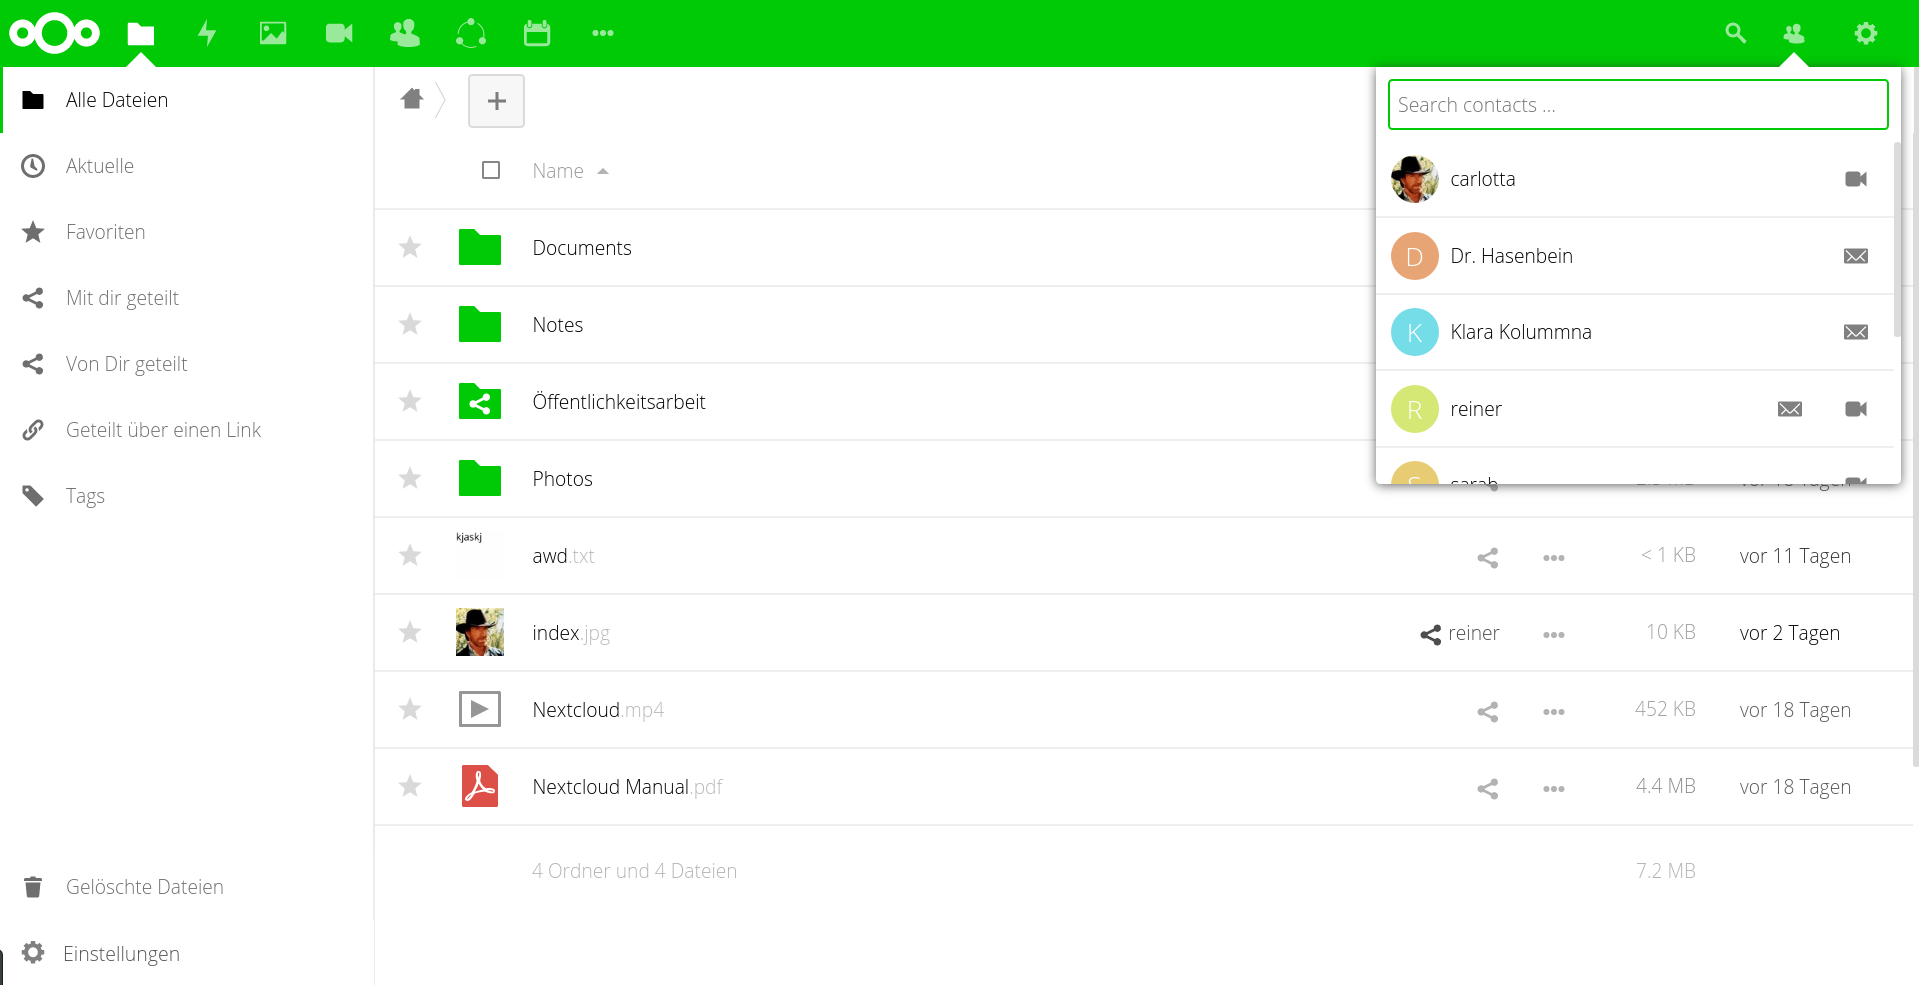
\includegraphics[width=\textwidth]{img/nextcloud1.png}
	\end{center}
\end{frame}
\note{Nextcloud ist eine gute Alternative für Dropbox, Google Calender/Contacts, Apple iCloud und Google Docs. Es kann alle diese Dinge, ist dabei aber Open Source und man kann sich wie bei Email seinen Anbieter (und damit den Ort wo seine Daten liegen, z.B. bei einem deutschen Anbieter in Deutschland) aussuchen. Wenn man ein bisschen Bescheid weiß, kann man sich sogar eine kleine Nextcloudbox zu Hause hinstellen oder es auf einem eigenen Webspace installieren um noch mehr Kontrolle über seine Daten zu haben.}

\begin{frame}{Nextcloud}
	\begin{center}
		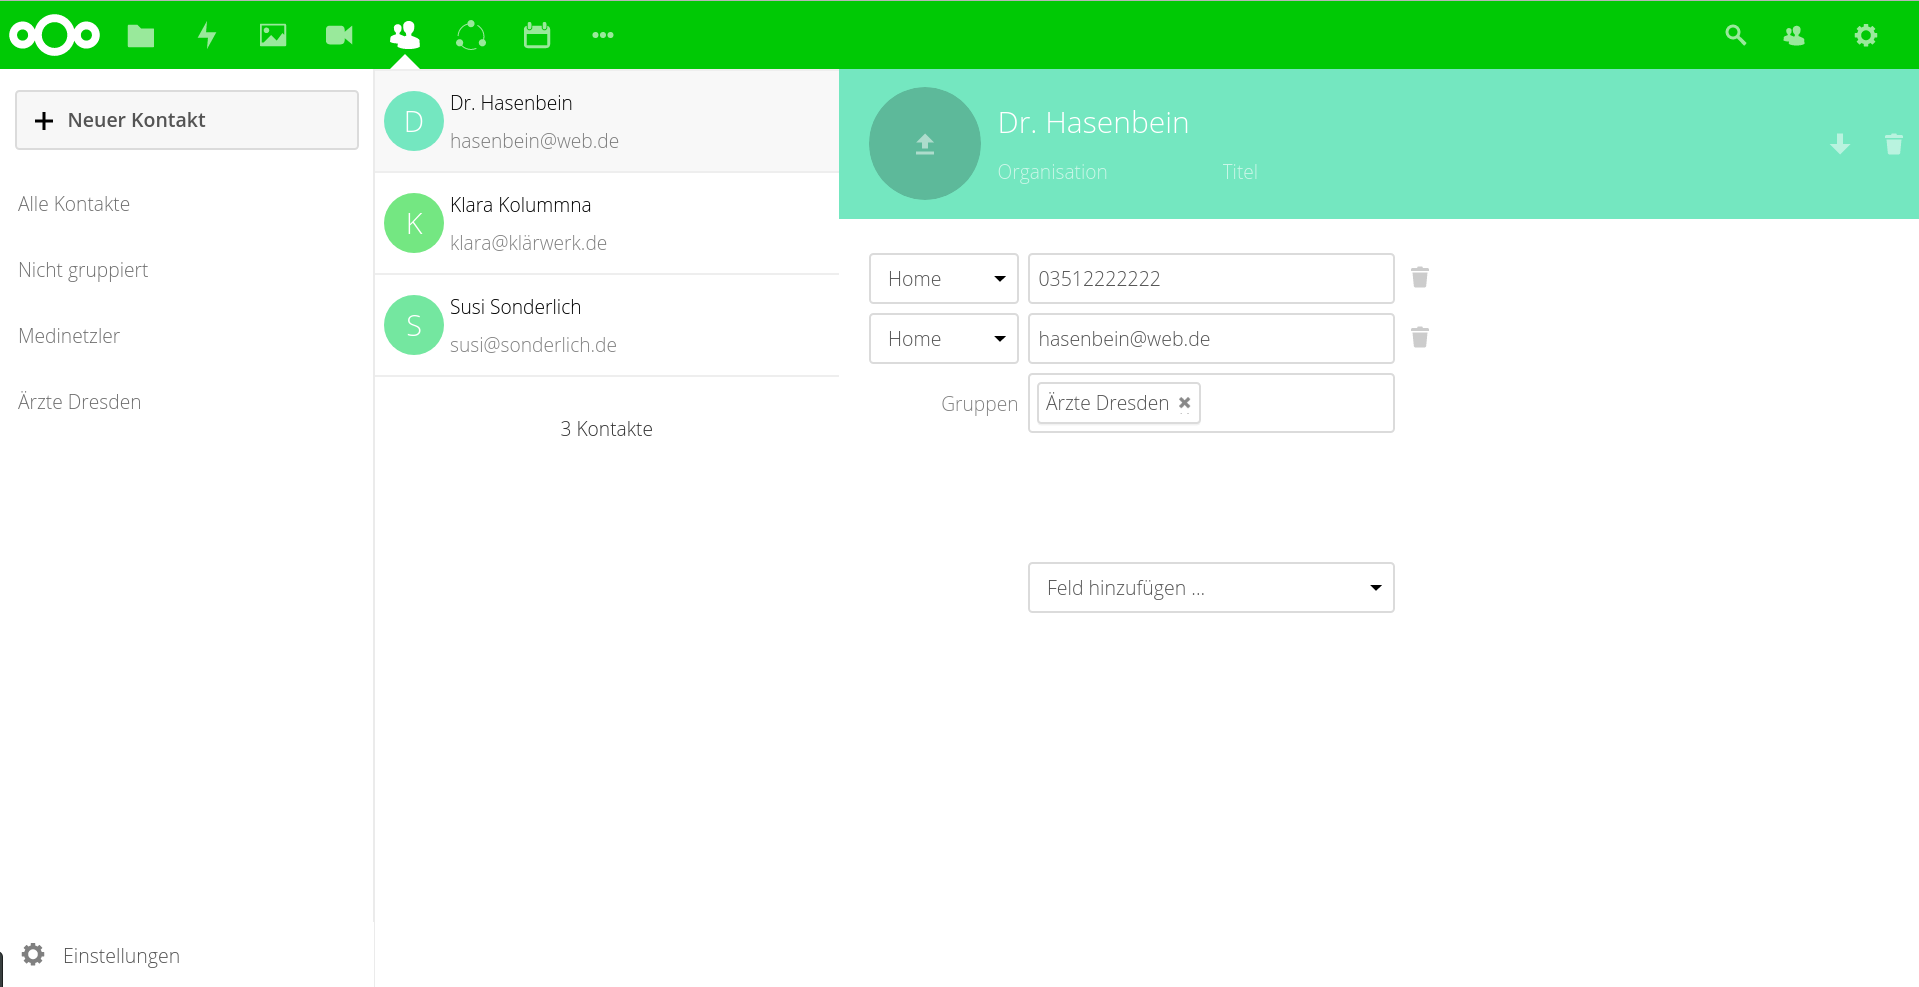
\includegraphics[width=\textwidth]{img/nextcloud2.png}
	\end{center}
\end{frame}

\begin{frame}{Nextcloud}
	\begin{center}
		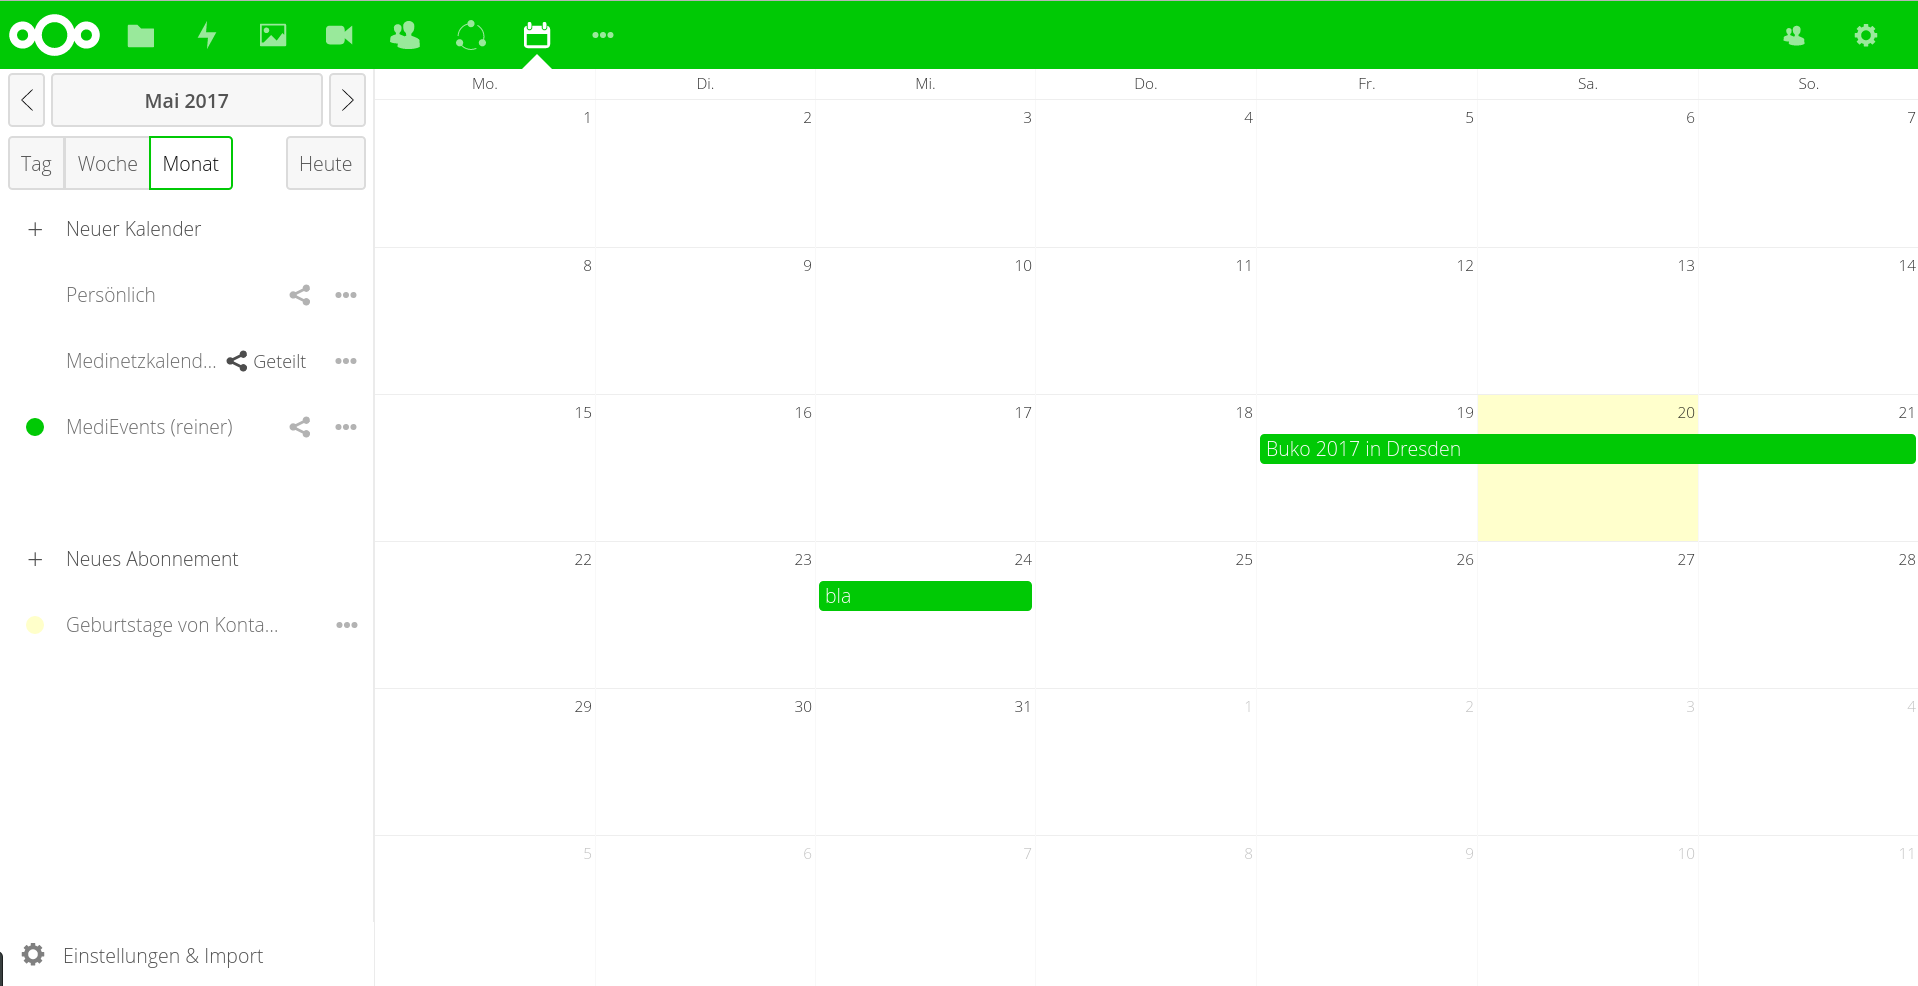
\includegraphics[width=\textwidth]{img/nextcloud3.png}
	\end{center}
\end{frame}

\begin{frame}{Nextcloud}
	\begin{center}
		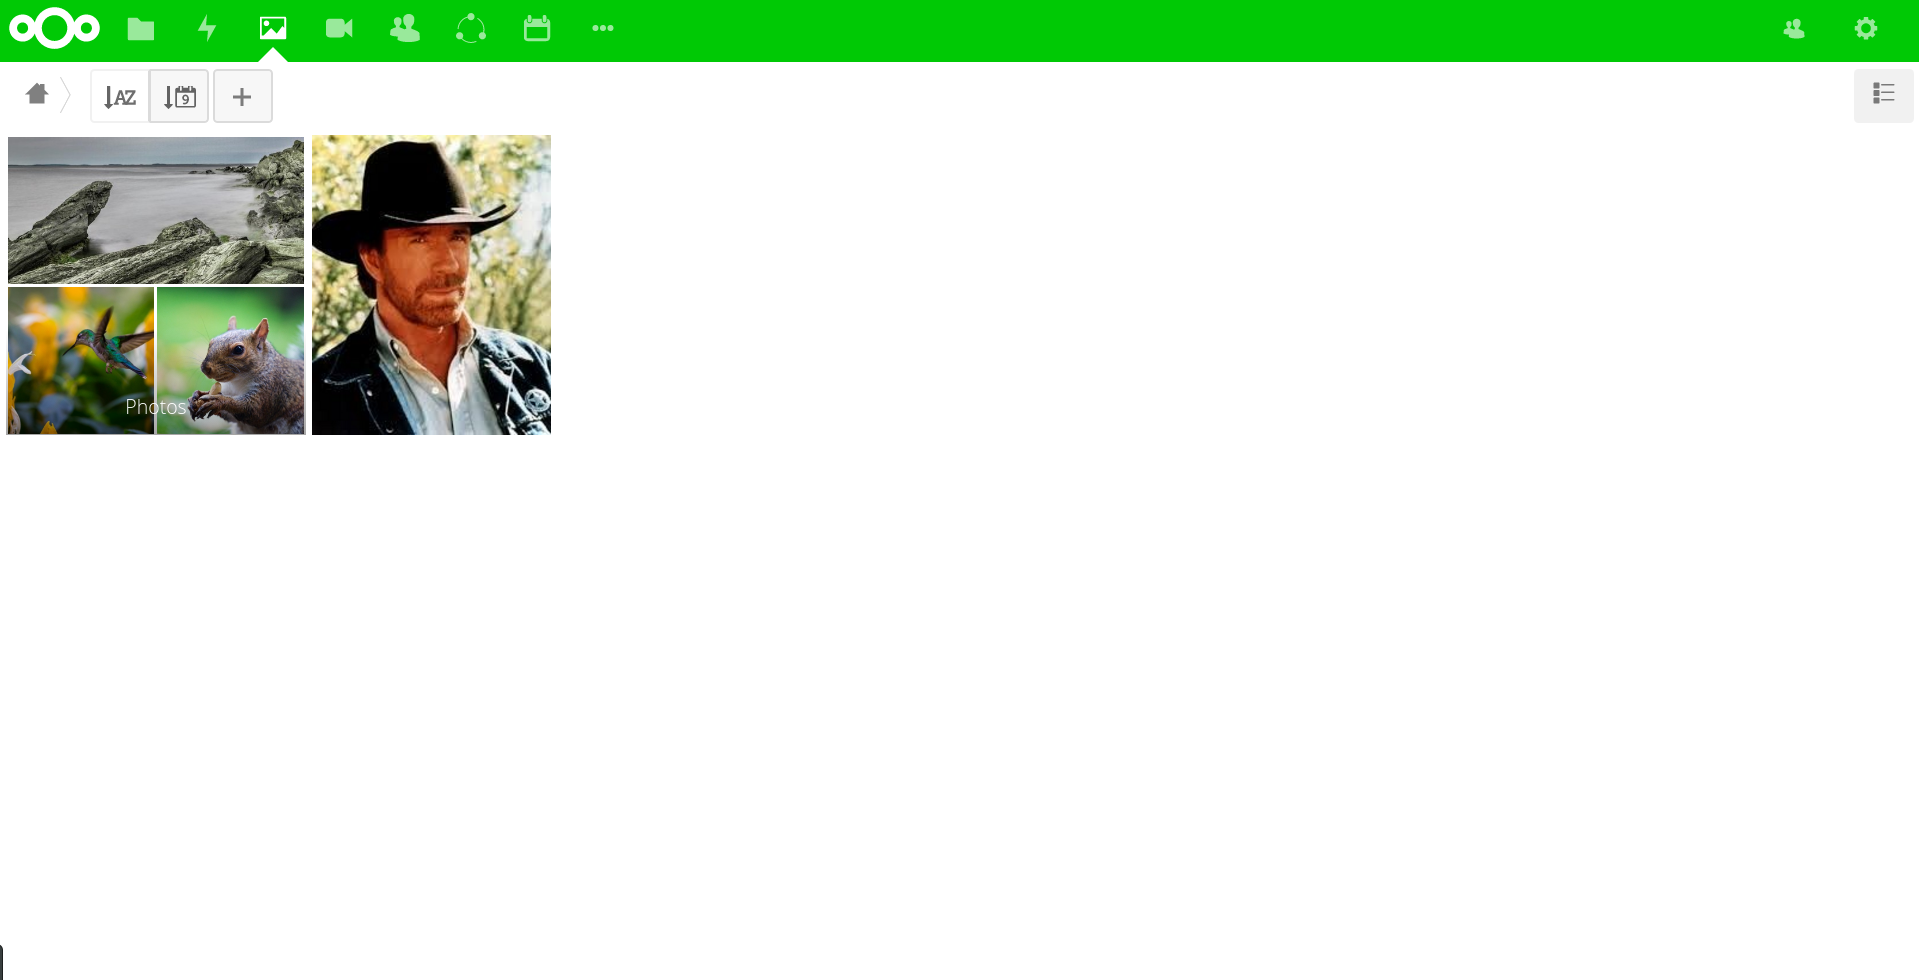
\includegraphics[width=\textwidth]{img/nextcloud4.png}
	\end{center}
\end{frame}

\begin{frame}{Nextcloud}
	\begin{center}
		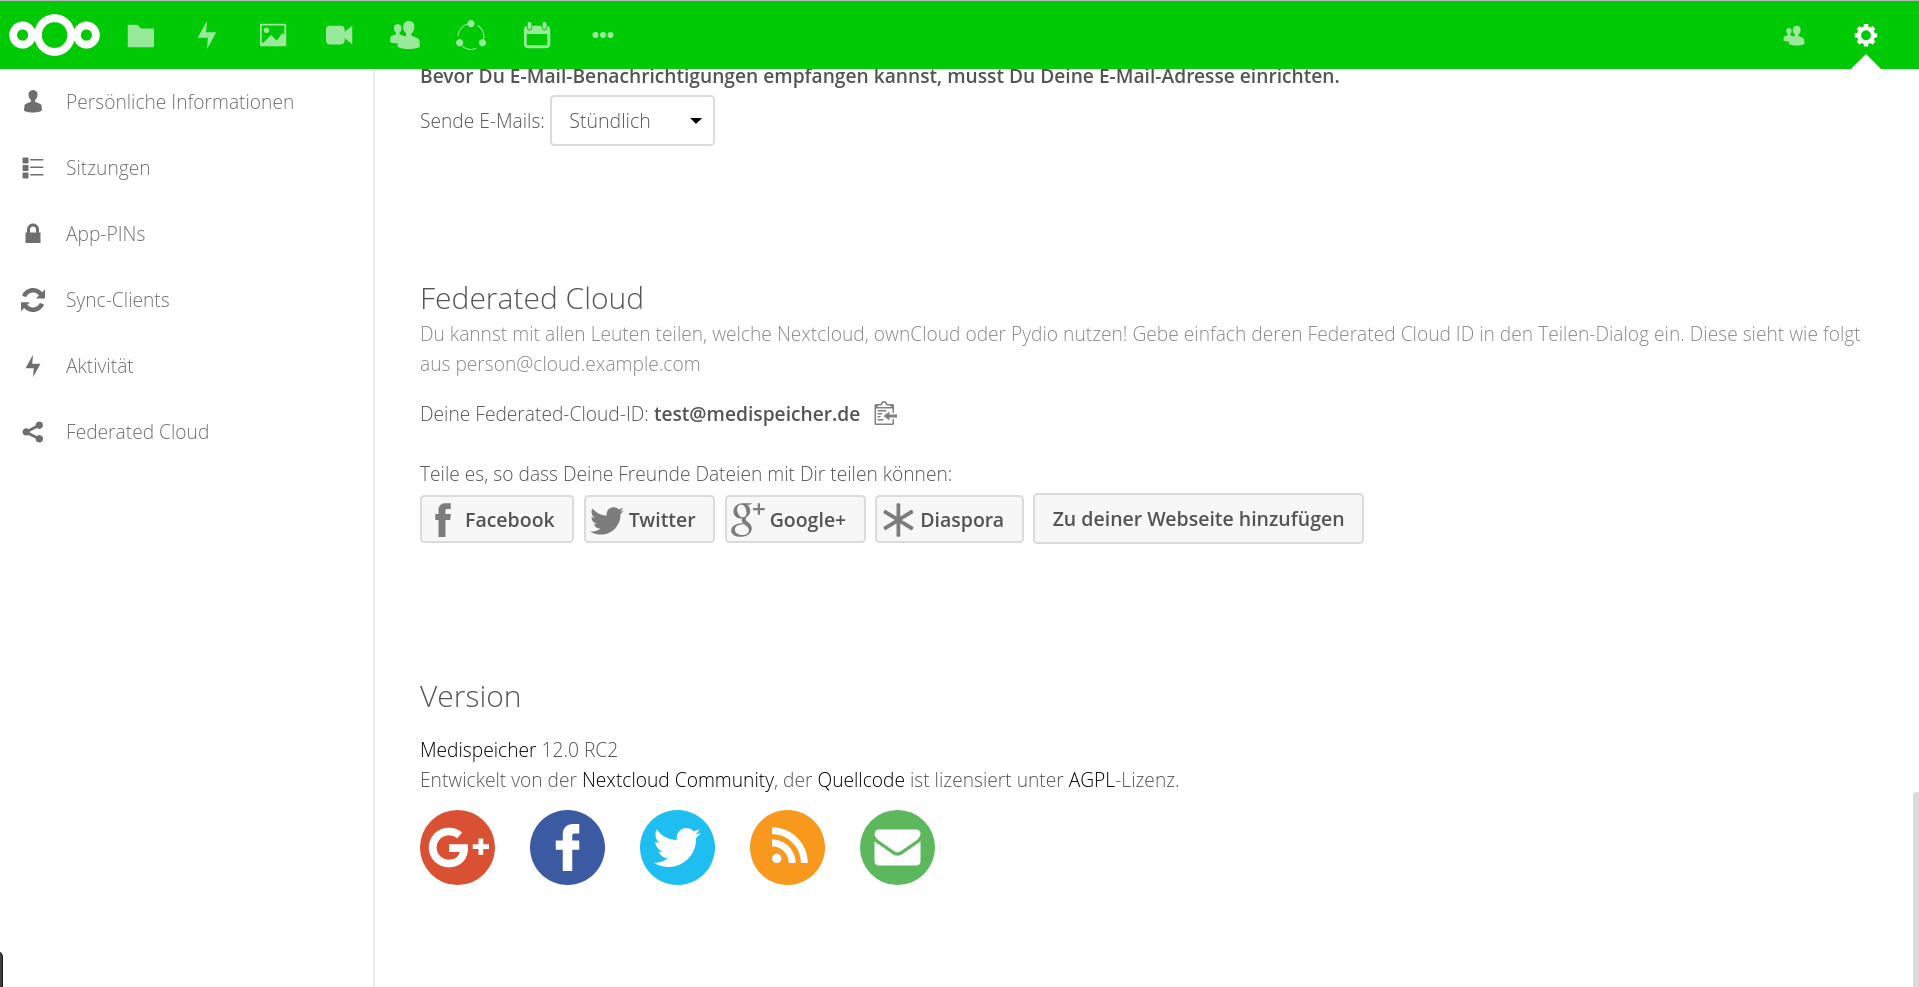
\includegraphics[width=\textwidth]{img/nextcloud5.png}
	\end{center}
\end{frame}

\begin{frame}{Nextcloud}
	\begin{center}
		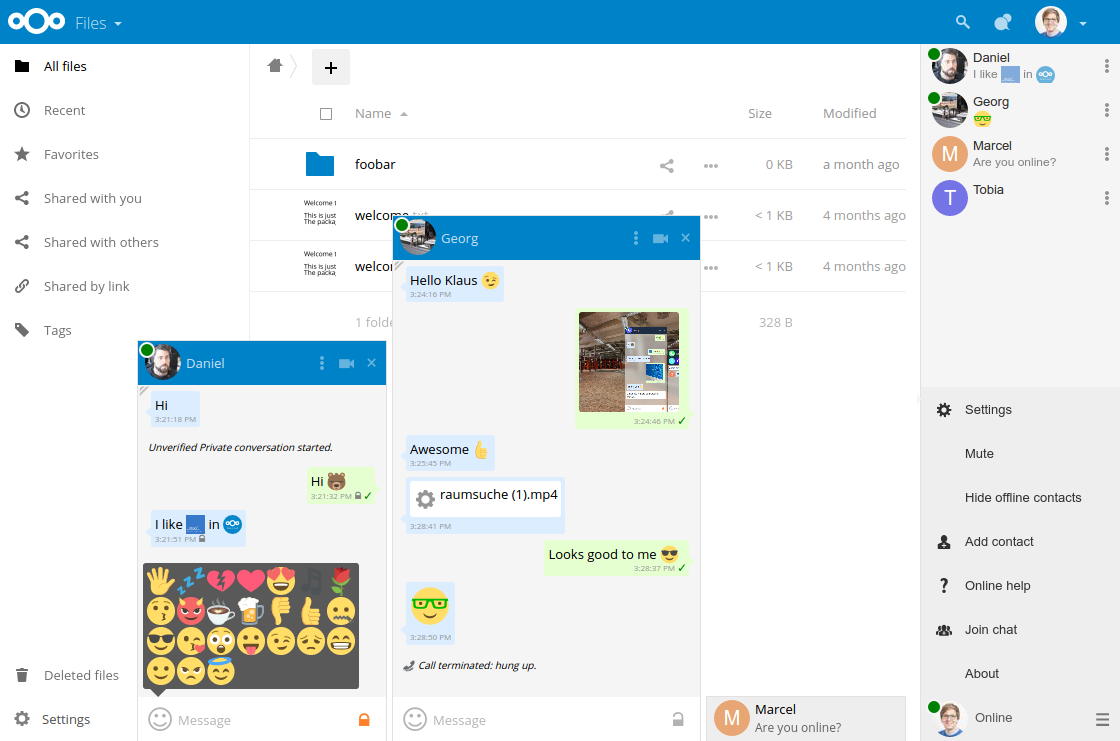
\includegraphics[width=\textwidth]{img/nextcloud6.png}
	\end{center}
\end{frame}
